\chapter{Background}

\section{Introduction}

Refactoring is the process of restructuring source code in order to improve the internal behavior
of the code, without changing the external behavior~\cite[9]{fowlerrefactoring}.
Refactoring on source code is often performed in order to eliminate instances of bad
design quality in code, otherwise known as code smells.

A study conducted by Diego Cedrim et al. has shown that while developers tend to refactor
smelly code, they are rarely successful at eliminating the smells they are
targeting~\cite{Rohit_Gheyi_Impact}. They also discovered that a large portion of
refactorings tend to make the code quality worse. Automated tools which help developers
make better refactorings and perform code analysis could be a solution to this problem.

Duplicated code is a code smell which occurs in practically every large software project.
Code clone analysis has recently become a highly active field of research and many tools
have been developed to detect duplicated code~\cite[7]{Inoue_introduction_to_cc}. However,
few of these have the capability of detecting intricate types of duplicated code and
managing them in a real-time IDE environment.

This thesis will present a tool and possibly techniques for clone detection and management
in real-time, which runs in modern IDE environments. The thesis will explore the topics
such as finding and managing clones in real-time, incremental analysis of source code and
providing clone management and refactoring tools in an editor and language
agnostic environment.

\section{Background}

\subsection{Software quality and duplicated code}

Software quality is hard to define. The term ``quality'' is ambiguous and is in the case
of software quality, multidimensional. Quality in itself has been defined as ``conformance
to requirements''~\cite[8]{crosby1980quality}. In software, A simple measure of
``conformance to requirements'' is a lack of bugs. However, software
quality is often measured in other metrics, including metrics which are not directly
related to functionality~\cite[29]{MetricsAndModelsInSoftwareQuality}. These metrics
often include maintainability, analyzability and changeability.

These metrics are affected negatively by duplicated code, code which is more or less
copied to different locations in the source code. Multiple studies have shown that
software projects typically contains $10-15\%$ duplicated code~\cite{CloningByAccident}.
Therefore, research into tools and techniques which can reduce duplicated code will be of
benefit to almost all software.

As stated, duplicated code damages software quality in software projects. Duplicated code
can lead to a plethora of antipatterns, and will often lead to an increase in technical
debt. Technical debt occurs when developers make technical compromises that are expedient
in the short term, but increases complexity in the long-term~\cite[111]{TechnicalDebt}. An
example of this in the context of duplicated code is the
``Shotgun-Surgery''~\cite[66]{fowlerrefactoring} antipattern. This antipattern occurs when
a developer wants to implement a change, but needs to change code at multiple locations
for the change to take effect. This is a typical situation which slows down development
and reduces maintainability when the amount of duplicated code increases in a software
project.

\subsection{Code clones}

Duplicated code is often described as ``code clones''.

\begin{definition}[Code snippet]
	A code snippet is a piece of contiguous source code in a larger software system.
\end{definition}

\begin{definition}[Code clone]
	A code clone is a code snippet which is equal to or similar to another code snippet. The two
	code snippets are both code clones, and together they form a code clone pair.
	Similarity is determined by some metric such as number of equal lines of code.
\end{definition}

\begin{definition}[Clone set]
	A clone set is a set of code snippets where all snippets are considered clones of each
	other.
\end{definition}

\subsubsection{Clone relation}

The clone relation is a relation between code snippets which defines pairs of clones.
The clone relation is reflexive and symmetric, but not always transitive. The transitive
property depends on the threshold for similarity when identifying code clones. Given

$$a \xleftrightarrow{clone} b \xleftrightarrow{clone} c$$


where $a,b,c$ are code snippets and $\xleftrightarrow{clone}$ gives the clone relation, $a$ is
a clone of $b$, but not necessarily similar enough to be a clone of $c$, depending on the
threshold for similarity.

If the threshold for similarity is defined such that only equal clones are considered
clones, the relation becomes transitive, and equivalence classes form clone sets.

\subsubsection{Code clone types}

Code clones are generally classified into four types~\cite{Inoue_introduction_to_cc}. The
types classify code snippets as code clones with an increasing amount of leniency.
Therefore, Type-1 code clones are very similar, while Type-4 clones are not necessarily
similar at all. When defining types, it is the syntactic and structural differences which
is compared, not functionality. The set of code clones classified by a code clone type
is also a subset of the next type, meaning all Type-1 clones are also Type-2 clones, but
not vice versa.

The code clone types are defined as follows:

\textbf{Type-1} clones are syntactically identical. The only differences allowed are elements
without meaning, like comments and white-space. Example:

\begin{tcolorbox}
	\begin{center}
		\begin{tabular}{c | c}
			\begin{lstlisting}
// Clone 1
for (int i = 0; i < 10;   i++) {
    print(i);
}
        \end{lstlisting} &
			\begin{lstlisting}
// Clone 2
for (int i = 0; i < 10; i++) {
    // A comment without meaning
    print(i);
}
        \end{lstlisting}
		\end{tabular}
	\end{center}
\end{tcolorbox}




\textbf{Type-2} clones are structurally identical. Possible differences include
identifiers, literals and types. Type-2 clones are relatively easy to detect by
consistently renaming identifiers and literals~\cite[2]{Zibran_real_time_search}. This
type of clone is relevant to consider in merging scenarios because this type
of clone is relatively simple to parameterize in order to merge two Type-2 clones.
Example:


\begin{center}
	\begin{tcolorbox}
		\begin{tabular}{c | c}
			\begin{lstlisting}
// Clone 1
for (int i = 0; i < 10; i++) {
    print(i);
}
    \end{lstlisting} &
			\begin{lstlisting}
// Clone 2
for (int (*\textbf j*) = (*\textbf 1*); (*\textbf j*) < 10; (*\textbf j++*)) {
    print((*\textbf j*));
}
    \end{lstlisting}
		\end{tabular}
	\end{tcolorbox}
\end{center}

\textbf{Type-3} clones are required to be structurally similar, but not equal. Differences
include statements which are added, removed or modified. This clone type relies on a
threshold $\theta$ which determines how structurally different snippets can be to be
considered Type-3 clones~\cite{Inoue_introduction_to_cc}. The granularity for this
difference could be based on differing tokens, lines, etc. Detecting this type of clone is
hard. Example:

\begin{tcolorbox}
	\begin{center}
		\begin{tabular}{c | c}
			\begin{lstlisting}
// Clone 1
for (int i = 0; i < 10; i++) {
    print(i);
}
\end{lstlisting} &
			\begin{lstlisting}
// Clone 2
for (int i = 0; i < 10; i++) {
    print(i);
    (*\textbf{int x = 10;}*)
}
\end{lstlisting}
		\end{tabular}
	\end{center}
\end{tcolorbox}




In this example there is a one line difference between the two snippets, so if $\theta
	\geq
	1$, the two snippets would be considered Type-3 clones.

\textbf{Type-4} clones have no requirement for syntactical or structural similarity.
Therefore, the only requirement is equal functionality. Detecting this type of clone is
very challenging, but attempts have been made using program dependency
graphs~\cite{SeedType4Detection}. The following example shows two code snippets which have
no clear syntactic or structural similarity, but is functionally equal:

\begin{tcolorbox}
	\begin{center}
		\begin{tabular}{c | c}
			\begin{lstlisting}
// Clone 1
print((n*(n-1))/2)

print(sum);
\end{lstlisting} &
			\begin{lstlisting}
// Clone 2
int sum = 0;
for (int i = 0; i < n; i++) {
    for (int j = i+1; j < n; j++) {
        sum++;
    }
}
print(sum);
\end{lstlisting}
		\end{tabular}
	\end{center}
\end{tcolorbox}


Type-1 clones are often referred to as ``exact'' clones, while Type-2 and Type-3 clones
are referred to as ``near-miss'' clones~\cite[1]{Zibran_real_time_search}.

\subsubsection{Code clone detection process and techniques}

\textbf{The Code clone detection process} is generally split into (but is not limited to)
a set of steps to identify clones~\cite{Inoue_introduction_to_cc}. This
process is often a pipeline of input-processing steps before finally comparing fragments
against each other and filtering. The steps are generally as follows:

\begin{enumerate}
	\item \textbf{Pre-processing}: Filter uninteresting code that we do not want to
	      check for clones, for example generated code. Then partition code into a set of
	      fragments, depending on granularity such as methods, files or lines.
	\item \textbf{Transformation}: Transform fragments into an intermediate
	      representation, with a source-map back to the original code.
	      \begin{enumerate}
		      \item Extraction: Transform source code into the input for the comparison
		            algorithm. Can be tokens, AST, dependency graphs, suffix tree, etc.
		      \item Normalization: Optional step which removes superficial differences such as
		            comments, whitespace and identifier names. Often useful for identifying type-2
		            clones.
	      \end{enumerate}
	\item \textbf{Match detection}: Perform comparisons which outputs a set of
	      candidate clone pairs.
	\item \textbf{Formatting}: Convert candidate clone pairs from the transformed
	      code back to clone pairs in the original source code.
	\item \textbf{Post-processing/Filtering}: Ranking and filtering manually or with
	      automated heuristics
	\item \textbf{Aggregation}: Optionally aggregating sets of clone pairs into clone sets
\end{enumerate}

Not all clone detection techniques will necessarily follow all these steps.

\paragraph{Matching techniques} are techniques which can be applied to match source-code to
detect clone-pairs. The matching technique will also require specific pre-processing to be
done in the earlier steps, for example creating an AST. Some of the most explored
techniques are as follows~\cite{ComparisonAndEvaluationOfTechniques}:

\paragraph{Text-based} approaches do very little processing on the source code before
comparing. Simple techniques such as fingerprinting or incremental hashing have been used
in this approach. Dot plots have also been used in newer text-based approaches, placing
the hashes of fragments in a dot plot for use in comparisons.

\paragraph{Token-based} approaches transform source code into a stream of tokens, similar to
lexical scanning in compilers. The token stream is then scanned for duplicated
subsequences of tokens. Since token streams can easily filter out superficial differences
such as whitespace, indentation and comments, this approach is more robust to such
differences. Concrete names of identifiers and values can be abstracted away when comparing
the token-stream, therefore Type-2 clones can easily be identified. Type-3 clones can also
be identified by comparing the fragments tokens and keeping clone pairs with a lexical
difference lower than a given threshold. This can be solved with dynamic
programming~\cite{BakerSparseDynamicProgramming}. A common approach to detect clones using
token-streams is with a suffix-tree. A suffix-tree can solve the \textit{Find all maximal
	repeats} problem efficiently, which in essence is the same problem as finding clone pairs.
This algorithm can also be improved to use a suffix-array instead, which requires less
memory.

\paragraph{Syntactic} approaches transform source code into either concrete syntax trees
or abstract syntax trees and find clones using either tree matching algorithms or
structural metrics. For tree matching, the common approach is to find similar subtrees,
which are then deemed as clone pairs. One way of finding similar subtrees is to hash
subtrees into buckets and compare them with a tolerant tree matching algorithm. Variable
names, literal values and other source may be abstracted to find Type-2 clones more
easily. Metrics-based techniques gather metrics for code fragments in the tree and uses
the metrics to determine if the fragments are clones or not. One way is to use
fingerprint functions where the fingerprint includes certain metrics, and compare the
fingerprints of all fragments to find clones.

\paragraph{Chunk-based} approaches decompose chunks of source code into signatures which are
compared. Chunk-size is based on selected granularity, which can be functions, blocks,
etc. Signatures can for example be based on some software metrics. Machine learning has
been used in this approach using methods as chunks and token-frequency within the method
as signature. A Deep Neural Network trained on this data can then be used to classify two
chunks as clone or non-clone~\cite{CCLearner}.

\paragraph{Hybrid} approaches combine multiple approaches in order to improve detection.
For example Zibran et al. developed a hybrid algorithm combining both token-based suffix
trees for Type-1 and Type-2 clone detection, with a k-difference dynamic programming
algorithm for Type-3 clone detection~\cite{Zibran_real_time_search}.

\subsection{Incremental editing and analysis}

While writing code, programmers usually only edit small portions of text at a time. One
``edit'' will therefore only affect small parts of the internal representations of the
code which most tools use to perform analysis. Reusing parts of this representation would
therefore be faster and allow programming tools to scale better.

\subsubsection{Incremental parsing}

Incremental parsing is the process of reparsing only parts of a syntax tree whenever an
edit is performed. The motivation behind incremental parsing is to have a readily
available syntax tree after every edit, while doing as little computing as possible to
build it.

Ghezzi and Mandrioli introduced in 1979 the notion of incremental parsing, and
introduced an incremental parser for LR $\land$ RL grammars. However, they were aware that
this algorithm was both slow and did not allow expressive enough
grammars.~\cite{IncrementalParsing}

Tim A. Wagner et al.~\cite{PracticalAlgorithmsForIncremental} later published a large work
on incremental software development environments, presenting many novel algorithms and
techniques for incremental tooling in programming environments.

``Tree-sitter'' is a parser generator tool which specializes in incremental parsing.
Inspired by Wagner's work, it supports incremental parsing, error recovery and querying
for specific nodes and subtrees~\cite{treesitter}. These features combined allow
Tree-sitter to become a powerful tool for analysis and has been used for editor features
such as syntax-highlighting, refactoring and code navigation.

\subsubsection{Incremental clone detection}

In order to incrementally detect code clones, an algorithm which first calculates the
initial code clones is run, and for successive revisions of the source code, this list is
incrementally updated, more efficiently than the initial run. Different approaches have
been used to accomplish this.

Göde and Koschke~\cite{GodeIncrementalCloneDetection} proposed the first incremental clone
detection algorithm. The algorithm employs a generalized suffix tree in which the amount
of work of updating is only dependent on the size of the edited code. This approach is
limited in scalability, as generalized suffix trees require a substantial amount of
memory.

Nguyen et al.~\cite{LocalitySensitiveHashingIncremental} showed that an AST-based approach
utilizing ``Locality-Sensitive Hashing'' can detect clones incrementally with high
precision, and showed that incremental updates could be done in real-time ($< 1$ second)
for source code with a size of 300 KLOC.

Hummel et al.~\cite{IndexBasedIncrementalCloneDetection} later introduced the first incremental,
scalable and distributed clone detection technique for Type-1 and Type-2 clones. This
approach utilizes a custom ``clone index'' data structure which can be updated
efficiently. The implementation of this data structure is similar to that of an inverted
index.


More recently, Ragkhitwetsagul and Krinke~\cite{SiameseScalableAndIncrementalClone}
presented the tool ``Siamese'', which uses a novel approach of having multiple
intermediate representations of source code to detect a high number of clones with
support for incremental detection. The tool can detect up to Type-3 clones, but will only
give clones based on ``queries'' given to it by the user. Queries are either files or
methods in source-code, which are then checked for existing code clone.

\subsection{IDE tooling}

\subsubsection{Existing IDE tools for clone management}

Developers are not always aware of the creation of clones in their code. Clone aware
development means having clone management as a part of the software development process.
Since code clones can be hard to keep track of and manage, tools which help developers
deal with clones are useful. However, Mathias Rieger et al. claims that a problem with
many detection tools is that the tools ``report large amounts data that must be treated
with little tool support''~\cite[1]{InsightsSystemWideDuplication}. Detecting and
eliminating clones early in their lifecycle with IDE integrated tools could be a solution
to the problem of dealing with too many clones.

There are many existing clone management tools, and the following section will go over
tools which are integrated into an IDE and offer services to the programmer while
developing in real-time.

The IDE-based tools which exist can be categorized as
follows~\cite[8]{Udding_Towards_Convenient_Management}:

\begin{itemize}
	\item\textit{Copy-paste-clones:} This category of tools deals only with code snippets which are
	copy-pasted from another location in code. These tools therefore only track clones which
	are created when copy-pasting, and does not use any other detection techniques. Therefore,
	this type of tool is not suitable for detecting clones which are made accidentally, since
	developers are aware that they are creating clones when pasting already existing code
	snippets.

	\item\textit{Clone detection and visualization tools:} This category of tools has more
	sophisticated clone detection capabilities and will detect code clones which occur
	accidentally.

	\item\textit{Versatile clone management:} This category of tools covers tools which provide more
	services than the above. Services like refactoring and simultaneous editing of clones fall
	under this category.
\end{itemize}

There are a few existing IDE-tools which have seen success in real-time detection of clones:

\begin{itemize}

	\item Minhaz et al. introduced a hybrid technique for performing real-time focused
	      searches, i.e. searching for code clones of a selected code snippet. This
	      technique can also detect Type-3 clones~\cite{Zibran_real_time_search}. It was
	      later used in the tool
	      \textit{SimEclipse}~\cite{Udding_Towards_Convenient_Management} which is a plugin
	      for the Eclipse editor. Since this tool can only detect clones of a code snippet
	      which the developer actively selects, this tool is not well suited for finding
	      accidental clones and tracking clones in areas.

	\item Another tool, SHINOBI, which is a plugin for the Visual Studio editor, can
	      detect code clones in real-time without the need of the developer to select a code
	      snippet. It can detect Type-1 and Type-2 code clones and uses a token-based suffix
	      array index approach to detect clones incrementally~\cite{SHINOBI}.

	\item The modern IDE IntelliJ has a built-in duplication detection and refactoring
	      service, it is able to detect Type-1 and (some) type-2 code clones at a method
	      granularity and refactors by replacing one of the clones with a method call to the
	      other.

\end{itemize}

\begin{figure}[t]
	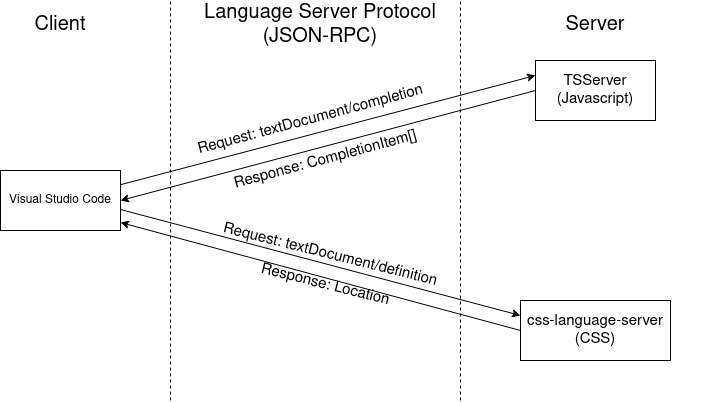
\includegraphics[width=\textwidth]{images/lspcommunication.png}
	\caption{Example client-server interaction using LSP}
	\label{fig:lspcommunication}
\end{figure}

\subsubsection{The Language Server Protocol}

Usually, static analysis tools which integrate with IDEs are tightly coupled to a specific
IDE and its APIs, like parsing and refactoring support. This makes the tools hard to
utilize a tool in another IDE, since the API's the tool utilizes is no longer available.
In order to make IDE-based static analysis tools more widely available, it would be
interesting to determine if such tools could be made editor agnostic.

The Language Server protocol (LSP) is a protocol which specifies interaction between a
client (IDE) and server in order to provide language tooling for the client. The goal of
the protocol is to avoid multiple implementations of the same language tools for every IDE
and every language, allowing for editor agnostic tooling. Servers which implement LSP will
be able to offer IDEs code-completion, error-messages, go-to-definition and more. LSP also
specifies generic code-actions and commands, which the LSP server provides to the client
in order to perform custom actions defined by the server.

Figure \ref{fig:lspcommunication} shows a sample interaction between client and server
using LSP. The client sends requests to a server in the form of JSON-RPC messages, and the
server sends a corresponding response, also in the form of JSON-RPC messages.

\section{Preliminary algorithms and data structures}

The following algorithms and data structures will be useful in following chapters to
describe the detection algorithm

% TODO add section about suffix trees here
\subsection{Suffix trees}

A classic algorithm for code clone detection traverses a suffix-tree in order to find
maximal repeats in all suffixes of the input string T.

\Tree[.IP [.NP [.Det \textit{the} ]
               [.N\1 [.N \textit{package} ]]]
          [.I\1 [.I \textsc{3sg.Pres} ]
                [.VP [.V\1 [.V \textit{is} ]
                           [.AP [.Deg \textit{really} ]
                                [.A\1 [.A \textit{simple} ]
                                      \qroof{\textit{to use}}.CP ]]]]]]

\subsection{Suffix arrays}

The suffix array (SA) of a string T contains a lexicographical sorting of all suffixes in T.
The suffix array does not contain the actual suffixes, but it contains integers pointing
to the index where the suffix starts in T. Conversely, the inverse suffix array (ISA)
contains integers describing which rank a suffix has. ISA[i] = n describes that the suffix
at position i in T, is the nth smallest suffix lexicographically.

\begin{definition}[Suffix array] 
    Let T be a text of length N.
    The suffix array SA of T is an array of length N where \texttt{SA[i] = n} if the
    suffix at \texttt{T[n..N-1]} is the ith smallest suffix in T lexicographically.

\end{definition}

\begin{definition}[Inverse suffix array] 
    Let T be a text of length N.
    The inverse suffix array ISA of T is an array of length N where \texttt{ISA[i] = n} if the
    suffix at \texttt{T[i..N-1]} is the nth smallest suffix in T lexicographically.
\end{definition}

\begin{table}
	\begin{center}
        \subfloat[Suffixes]{
		\begin{tabular}{c | l }
			Index & Suffix   \\
			\hline
			0     & BANANA\$ \\
			1     & ANANA\$  \\
			2     & NANA\$   \\
			3     & ANA\$    \\
			4     & NA\$     \\
			5     & A\$      \\
			6     & \$       \\
    \end{tabular}}
		\hspace{1cm}
        \subfloat[Sorted suffixes]{\begin{tabular}{c | l}
			Index & Suffix   \\
			\hline
			6     & \$       \\
			5     & A\$      \\
			3     & ANA\$    \\
			1     & ANANA\$  \\
			0     & BANANA\$ \\
			4     & NA\$     \\
			2     & NANA\$   \\
    \end{tabular}}
		\hspace{1cm}
        \subfloat[SA and ISA]{\begin{tabular}{c | c | c}
				Index & SA & ISA \\
				\hline
				0     & 6  & 4   \\
				1     & 5  & 3   \\
				2     & 3  & 6   \\
				3     & 1  & 2   \\
				4     & 0  & 5   \\
				5     & 4  & 1   \\
				6     & 2  & 0   \\
        \end{tabular}}
		\caption{T=BANANA\$}
        \label{table:BANANA}
	\end{center}
\end{table}

Table \ref{table:BANANA} shows the suffix array of a text T=BANANA\$ and the correlation
between the sorted suffixes and the suffix array.

% TODO describe LCP array here

% TODO add correlation between suffix array and tree here with applications

Suffix arrays can be constructed in linear time in terms of the length of T. Many
so-called suffix array construction algorithms (SACA) have been discovered in the last
decade\cite{SuffixArrayConstruction}, many of which run in linear-time. An algorithm
which has been shown to be very efficient in practice is Nong and
Chan's.\cite{LinearTimeSuffixArraySAIS} algorithm based on induction sorting.

% TODO, describe this algorithm more here


\subsection{Burrows-wheeler transform}

% TODO write about BW transform

\subsection{Dynamic suffix arrays}

% Write about dynamic SA's

\subsection{Incremental-parsing and error-recovery}

% Write about incremental parsing algorithms here


\section{The way forward}

This thesis will present and evaluate a tool which provides clone management
capabilities in a real-time IDE environment. The main goal will be to create a tool which
fits well into the development cycle and works in a real-time IDE environment. Areas of
focus will therefore be:

\begin{itemize}
	\item Code clone detection
	\item Real-time / Incremental detection of code clones
	\item IDE agnostic tooling like LSP and Tree-sitter
	\item Possibly clone ranking, determining which clones should be kept.
\end{itemize}

\subsection{LSP for IDE-based clone management}

The tool will give programmers the ability to manage clones in their IDE. We will utilize
many feature of LSP, especially code-actions, in order to provide functionality for clone
management to any editor which implements LSP.

The following user stories shows how interaction with the LSP server will work.

\begin{itemize}
	\item A programmer wants to see code clones for a file, the
	      programmer opens the file in their IDE and is displayed diagnostics in the code
	      wherever there are detected clones. The matching code clones are not necessarily
	      in the same file.

	\item A programmer wants to see all code clones for the current project. The
	      programmer opens the IDEs diagnostic view and will see all code clones detected
	      as diagnostics there. The diagnostic will contain information like where the clone
	      exists, and percentage of duplicated code.

	\item A programmer wants to jump to the corresponding match of a code clone in their
	      editor. The programmer moves their cursor to the diagnostic and will see a list of
	      the matching code clones. The programmer will select the wanted code clone which
	      will move the cursor to the file and location of the selected code clone.

	\item A programmer wants to merge a code clone pair. The programmer moves their cursor
	      to one of the code clones, invokes a request to see code actions, and invokes one
	      of the ``Merge code clone with strategy x`` actions. The strategies presented to
	      the user are dependent on the context of the code clone pair, the programmer will
	      only see the useful / realizable merging strategies.
\end{itemize}

The interaction with the LSP server will depend on the client's implementation of LSP. If
the LSP client is limited in its capabilities, meaning it does not implement the entire
protocol, the tool will be limited in how the programmer can interact with it.

\subsection{Architecture of tool}

Figure \ref{fig:architecture} shows the architecture of the tool. The server communicates
with the IDE and delegates the work of managing clones to the detection engine and the
merge engine. The tool also stores an index of all source code files in the current project.

\subsection{Exploring clone management techniques}

During development of the tool, different techniques for detecting clones will be
explored. The goal will be to find a fitting technique for both detecting and merging
clones in a real-time IDE environment.

Detection techniques explored will include:

\begin{itemize}
	\item A fully incremental version of Zibran et al. hybrid
	      algorithm~\cite{Zibran_real_time_search}
	\item AST-based technique with incremental parsing. Using Tree-sitter to parse and an
	      incremental detection algorithm to detect clones.
\end{itemize}

\begin{figure}
	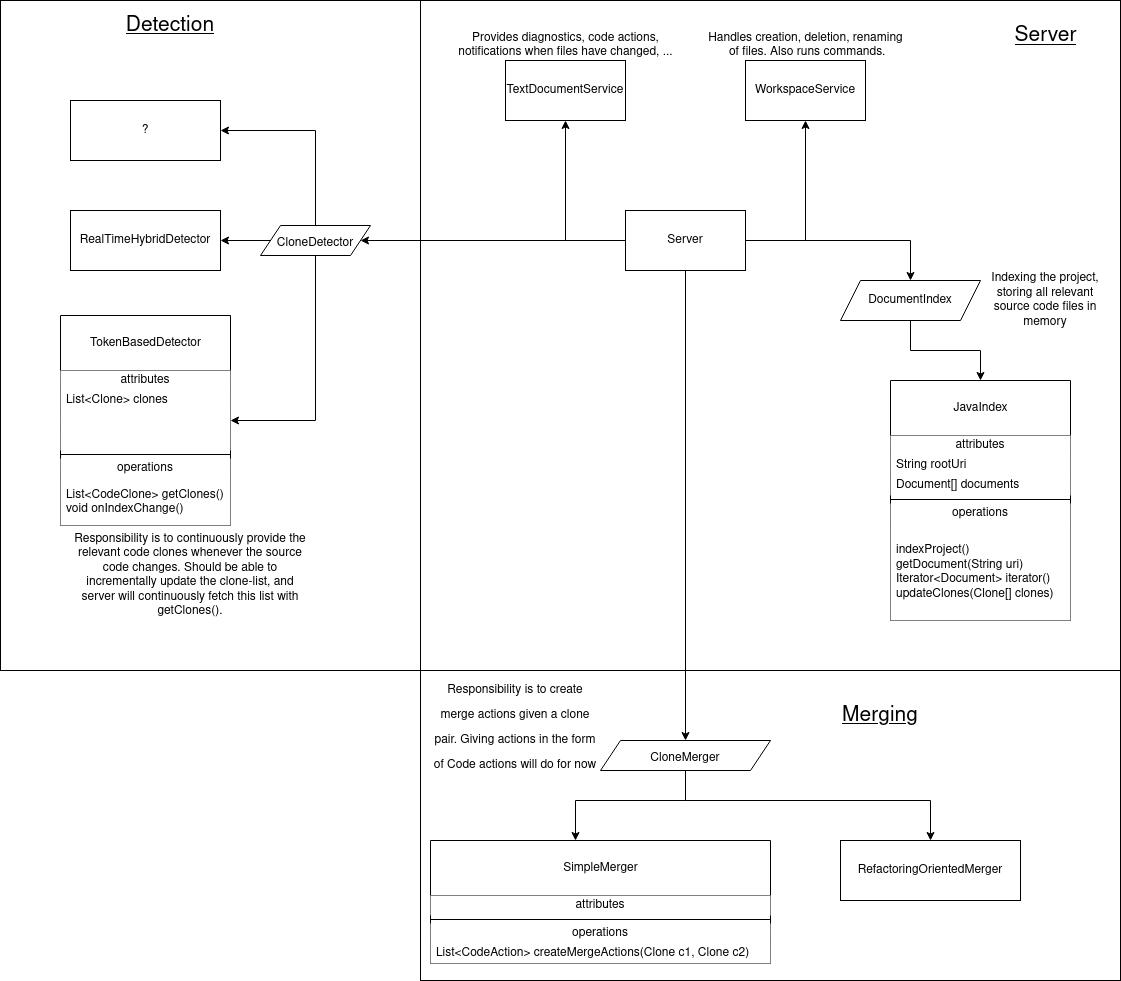
\includegraphics[width=\textwidth]{images/ToolArchitecture.png}
	\caption{Tool architecture}
	\label{fig:architecture}
\end{figure}

The tool will be modular in how techniques are applied for clone management. This
means that the tool will be capable of plugging in different detection engines, merging
engines and file indices. This will be used extensively in our research in order to test
multiple techniques for detection and merging.

\subsection{Evaluation}

We will evaluate this tool based on different criteria, which combined will provide a
basis for evaluating the tool as a whole.

Since the tool is focused on efficient detection and management of code clones, real-time
performance of the tool will be a high priority in its evaluation. The tool will implement
different techniques of detecting and merging clones. These will be empirically compared
against each other. The tool will also be evaluated against existing tools empirically. We
will utilize BigCloneBench~\cite{BigCloneBench} to evaluate detection techniques, by
running our detection techniques in a standalone mode. We will distinguish between initial
detection and incremental detection when evaluating.

The tool will also be evaluated in how well it fits into the software development cycle.
Can we determine if this tool is an effective way to detect a clone early in its lifecycle
so that they can be removed before it manifests in the source code? In relation to this,
we will evaluate if LSP is a suitable tool for use in clone management and refactoring in
general. Can LSP provide all the features one would want in a modern analysis tool? What
is missing, and how could the LSP protocol be extended in order to facilitate this? We
believe that if LSP is an appropriate tool to use for clone management, LSP will also be
an appropriate tool for static analysis tools in general.


